\chapter{Teorema di Gauss-Green, del flusso e del rotore}
In questo capitolo enunciamo questi importanti risultati, che hanno grandissima applicazione. Alcune dimostrazioni non sono state fatte a lezioni e sono riportati i libri in cui possono essere consultate. 
\section{Teorema di Gauss-Green}
Vogliamo adesso ricavare il teorema di Gauss-Green, il quale ci consente di ricavare un altro modo per determinare la misura degli insiemi nel piano e consente di ottenere le cosiddette \emph{forme differenziali d'area}, che rappresentano, in un certo senso, l'elemento infinitesimo di area. Per dimostrare il teorema
abbiamo bisogno di qualche definizione preliminare.
\begin{theorem}[curva semplice]
	$\varphi: [a, b] \to \mathbb{R}^2$ è semplice se $\gamma|_{[a, b)}$ e $\gamma|_{(a, b]}$ sono iniettive.
\end{theorem}
\begin{remark}
	Una curva semplice può essere chiusa: se $\gamma(a) = \gamma(b)$ allora $\gamma|_{(a, b]}$ e $\gamma|_{[a, b)}$.
\end{remark}
\begin{remark}
	Se $\gamma: [a, b] \to \mathbb{R}^2, \gamma|_{[a, b)}$ è iniettiva allora non può essere semplice: infatti potrebbe esistere un punto $c \in (a, b)$ tale che
	$\gamma(b) = \gamma(c)$ allora $\gamma|_{[a, b)}$ e $\gamma|_{(a, b]}$.
\end{remark}
\begin{definition}[aperto regolare]
	Sia $\Omega \subseteq \mathbb{R}^2$ un insieme aperto, connesso per archi e limitato. Se supponiamo che $\text{Fr}\Omega$ sia un'unione di curve chiuse, semplici e $C^1_\text{tratti}$ diremo che
	è un aperto regolare e denoteremo la sua frontiera con il simbolo $\partial \Omega$, detto \emph{bordo di} $\Omega$.
\end{definition}
\begin{definition}[orientazione del bordo regolare]
	Sia $\Omega$ un insieme regolare e siano $\gamma_1, \ldots, \gamma_N$ le curve semplici, chiuse e $C^1_\text{tratti}$ le cui immagini costituiscono $\partial \Omega$. Se tutte le curve $\gamma_i$ percorrono
	$\partial \Omega$ lasciando $\Omega$ alla sua sinistra, diremo che orientano positivamente $\Omega$, altrimenti lo orientano negativamente. \\
	Indicheremo con $\partial^{+} \Omega$ il bordo di $\Omega$ positivamente orientato, mentre con $\partial^{-} \Omega$ il bordo di $\Omega$ negativamente orientato.
\end{definition}
Tramite questa definizione, possiamo dare un senso all'integrale curvilineo calcolato sul bordo positivamente orientato

\begin{definition}[integrale curvilineo sul bordo positivamente orientato]
	Sia $\Omega \subseteq \mathbb{R}^2$ un aperto regolare e sia $\partial^{+} \Omega$ il bordo positivamente orientato dalle curve $\gamma_1, \ldots, \gamma_N$ $C^1_\text{tratti}$, semplici e chiusi; ove
	$\gamma_i: [a_i, b_i] \to \partial \Omega \, \, \forall i \in \{1, \ldots, N \}$. Sia $\omega \in C^0(\mathcal{U}, (\mathbb{R}^2)^*)$ una $1-$forma differenziale ove $\partial \Omega \subseteq \mathcal{U} \subseteq \mathbb{R}^2$. \\
	Definiamo allora
	$$
	\int_{\partial^{+} \Omega} = \sum_{i=1}^N \int_{\gamma_i} \omega = \sum_{i=1}^N \int_{a_i}^{b_i} \omega(\gamma(t))(\dot{\gamma}(t))dt
	$$
	Se $\Gamma_i: [\alpha_i, \beta_i] \to \partial \Omega$ sono delle curve $C^1_\text{tratti}$, semplice e chiuse che orientano negativamente il bordo $\partial \Omega$ definiamo
	$$
	\int_{\partial^{-} \Omega} = \sum_{i=1}^N \int_{\Gamma_i} \omega = \sum_{i=1}^N \int_{\alpha_i}^{\beta_i} \omega(\Gamma(t))(\dot{\Gamma}(t))dt
	$$
\end{definition}
\begin{remark}
	Gli integrali $\int\limits_{\partial^{+} \Omega} \omega, \int\limits_{\partial^{-} \Omega} \omega$ non dipendono dalla scelta della parametrizzazione delle curve chiuse, semplici e $C^1_\text{tratti}$ che parametrizzano il bordo, ma solo dal
	loro verso di percorrenza. Questo è una proprietà dell'integrale curvilineo di seconda specie (teorema di invarianza). \\
	Si può inoltre osservare che
	$$
	\int_{\partial^{+} \Omega} \omega = - \int_{\partial^{-} \Omega} \omega
	$$
\end{remark}
\begin{theorem}[di Gauss-Green nel piano]
	Sia $\Omega \subseteq \mathbb{R}^2$ un aperto regolare e $F \in C^1(\bar{\Omega}, \mathbb{R}^2)$. Allora
	$$
	\int_\Omega \left( \frac{\partial F_2}{\partial x} - \frac{\partial F_1}{\partial y} \right) dxdy = \int_{\partial^{+} \Omega} F_1dx + F_2dy
	$$
\end{theorem}
\begin{proof}[Dimostrazione euristica]
	Vediamo l'integrazione lungo il bordo $\partial \Omega$ come orientata $"dx \wedge dy"$:
	\begin{align*}
	&\int_\Omega \left(\frac{\partial F_2}{\partial y} - \frac{\partial F_1}{\partial x} \right) dx \wedge dy = \int_\Omega \frac{\partial F_2}{\cancel{\partial x}} \cancel{dx} \wedge dy - \int_{\Omega} \frac{\partial F_1}{\partial y} dx \wedge dy = \\
	&=\int_{\partial^{+} \Omega} F_2 dy + \int_{\partial^{-} \Omega} \frac{\partial F_1}{\cancel{\partial y}} \cancel{dy} \wedge dx = \int_{\partial^{+} \Omega} F_2 dy + \int_{\partial^{+} \Omega} F_1 dx
	\end{align*}
	dove la penultima eguaglianza si è ottenuta osservando che dobbiamo "invertire" $dx \wedge dy$ ma geometricamente percorrere un bordo positivamente o negativamente cambia solamente il segno, dunque $dx \wedge dy = - dy \wedge dx$ (rimando alle appendici per una trattazione più accurata del prodotto \emph{wedge}).
\end{proof}
\begin{example}
	Sia $\Omega = (-1, 1) \times (1, 2)$ e sia $F=(x^2 - y, x^2 - y)$. Sia inoltre $\gamma$ una curva semplice, chiusa e $C^1_\text{tratti}$ che percorre $\partial \Omega$ in senso orario. Determinare
	$$
	\int_\gamma F
	$$
\end{example}
\begin{proof}
	Il valore dell'integrale lungo il bordo è, ovviamente, indipendente dalla parametrizzazione. Conseguentemente potremmo pensare di applicare il teorema di Gauss-Green sulla curva semplice, chiusa e $C^1_\text{tratti}$ più "semplice" possibile, ovvero una curva di forma rettangolare.
	Pertanto
	\begin{flalign*}
	&\int_{\gamma} F = -\int_{\partial^{+} \Omega} F = - \int_{\partial^{+} \Omega} F_1 dx + F_2 dy = - \int_\Omega \left( \frac{\partial F_2}{\partial x} - \frac{\partial F_1}{\partial y} \right) dxdy = \\ 
	&\int_{-1}^{1} dx \int_1^2 (-1 - 2x)dy = \int_{-1}^{1} (-1 - 2x)dx = -2 - 2 \int_{-1}^1 xdx = -2 \implies \int_{\gamma} F = - 2
	\end{flalign*}
\end{proof}
\begin{example}
	Sia $\gamma(t) = \begin{pmatrix} \cos{t}, & \frac{\sin{t}}{\sqrt{2}} \end{pmatrix}, \gamma: [0, 2\pi] \to \mathbb{R}^2$. Calcolare $\int_\gamma \eta_0$, dove $\eta_0 = - \frac{y}{x^2 + y^2}dx + \frac{x}{x^2 + y^2}dy$.
\end{example}
\begin{proof}
	$$\int_{0}^{2\pi} \left(\frac{1}{\sqrt{2}} \frac{\sin^2{t}}{\cos^2{t} + \frac{1}{2} \sin^2{t}} + \frac{1}{\sqrt{2}} \frac{\cos^2{t}}{\cos^2{t} + \frac{1}{2} \sin^2{t}} \right)dt = \frac{1}{\sqrt{2}} \int_0^{2\pi} \frac{1}{\cos^2{t} + \frac{1}{2} \sin^2{t}}dt$$. Osserviamo che, nonostante questo integrale non sia risolvibile, abbiamo un grande problema: la funzione non è definita su
	$$
	E = \{(x, y) \in \mathbb{R}^2 : x^2 + 2y^2 < 1 \}
	$$
	che è un insieme aperto, regolare e orientato positivamente da $\gamma$, tuttavia $\eta_0$ non è definita in $(0, 0)$ e non è possibile estenderla con continuità. \\
	Possiamo però restringere l'insieme a
	$$
	H = E \setminus \mathbb{B}(0, \frac{1}{2})
	$$
	che è un aperto regolare, dove $\eta_0 \in C^1(\mathcal{U}, (\mathbb{R}^2)^*), \bar{H} \subseteq U \subseteq \mathbb{R}^2$ e posso applicare Gauss-Green ad $\eta_0$ sull'aperto $H$: definiamo
	\begin{align*}
		&F_1=-\frac{y}{x^2 + y^2}	&	F_2 = \frac{x}{x^2 + y^2} &
	\end{align*}
	e osserviamo che, come avevamo visto già in precedenza, $\eta_0$ è chiusa $\implies \frac{\partial F_2}{\partial x} = \frac{\partial F_1}{\partial y}$, dunque
	$$
	\int_H \left(\frac{\partial F_2}{\partial x} - \frac{\partial F_1}{\partial y} \right) = 0 = \int_{\partial^{+} H} F_1 dx + F_2 dy \implies  \int_{\partial^{+} H} \eta_0 = 0 = \int_\gamma \eta_0 + \int_c \eta_0
	$$
	dove $\gamma$ è la curva che orienta positivamente il bordo, mentre la curva $c$ orienta positivamente il bordo interno (dovuto alla rimozione della palla centrata in $0$ e di raggio $2$). Ma allora
	$$
	\int_\gamma \eta_0 = - \int_c \eta_0
	$$
	possiamo parametrizzare $\tilde{c}(t) = \frac{1}{2} \begin{pmatrix} \cos{t}, & \sin{t} \end{pmatrix}$ che si muove in senso antiorario, da cui ricaviamo che
	$$
	\int_{\tilde{c}} \eta_0 = 2\pi \implies \int_\gamma \eta_0 = - \int_c \eta_0 = \int_{\tilde{c}} \eta_0
	$$
\end{proof}
\subsection{Forme differenziali d'area}
\begin{prop}
	Sia $H \subseteq \mathbb{R}^2$ un aperto regolare. Allora
	$$
	m_2(H) = \int_H 1dxdy = \int_{\partial^{+} H} xdy = - \int_{\partial^{+} H} ydx = \int_{\partial^{+} H}	 \frac{xdy - ydx}{2}
	$$
\end{prop}
\begin{proof}
Preso $F_1=y$ e $F_2 = 0$ avremo che
$$
\int_H 1dxdy = -\int_{\partial^{+} H} ydx
$$
e preso $F_1 = 0$ e $F_2 = x$ avremo che
$$
\int_H 1dxdy = \int_{\partial^{+} H} xdy
$$
dunque
$$
m_2(H) = \int_H 1dxdy = \int_{\partial^{+} H} \frac{xdy - ydx}{2} 
$$
\end{proof}
Un'operazione molto utile che possiamo fare è il cosiddetto \emph{pull-back} di una forma differenziale rispetto a delle coordinate: questo è particolarmente interessante per le forme differenziali di un'area, le quali rappresentano, in un certo senso, l'elemento infinitesimo di area.
\begin{definition}[pull-back di una $1-$forma differenziale]
	Sia $T$ una funzione differenziabile tale che $T: \mathcal{V} \to \mathcal{U}$ e $\omega$ una $1-$forma differenziale tale che $\omega \in C^0(\mathcal{U}, (\mathbb{R}^n)^*) \implies$
	$$
	T^*\omega \in C^0(\mathcal{V}, (\mathbb{R}^n)^*)
	$$
\end{definition}
\begin{remark}
	Il nome antisonante deriva proprio dal fatto che sto tirando indietro la $1-$forma differenziale da $\mathcal{U}$ a $\mathcal{V}$
\end{remark}
Un'interessante proprietà del pull-back è la seguente:
$$
\int_\gamma \omega = \int_{T^{-1} \circ \gamma} T^*\omega
$$
\begin{example}[forma d'area in coordinate polari]
	Sia $T(\rho, \varphi) = \begin{pmatrix}	\rho \cos{\varphi} & \rho \sin{\varphi} \end{pmatrix}$ con $\rho > 0, 0 < \varphi < 2\pi$. Vogliamo determinare $T^*\omega$ dove, naturalmente, $\omega = \frac{xdy-ydx}{2}$. Il calcolo si ottiene, banalmente, sostituendo al posto di $x$ e $y$ le nuove "espressioni", calcolandone
	naturalmente il differenziale
	\begin{align*}
	&\frac{xdy - ydx}{2} = \frac{\rho \cos{\varphi} d(\rho \sin{\varphi}) - \rho \sin{\varphi} d(\rho \cos{\varphi})}{2} = & \\ 
	&\frac{1}{2} \left( \rho \cos{\varphi} \sin{\varphi} d\rho + \rho^2 \cos^2{\varphi} d\varphi - \rho \sin{\varphi} \cos{\varphi} d\rho + \rho^2 \sin^2{\varphi} d\varphi \right) = \frac{1}{2} \rho^2 d\varphi
	\end{align*}
	dunque $T^*\omega = \frac{1}{2} \rho^2 d\varphi$ è la $1-$forma differenziale d'area in coordinate polari, definita in $(0, +\infty) \times (0, 2\pi)$. Siamo adesso autorizzati a dire che
	$$
	d\sigma = \frac{1}{2} \rho^2 d\varphi
	$$
\end{example}
\begin{example}[area di una regione tramite la $1-$forma d'area in coordinate polari]
	Consideriamo $E = \{(\rho \cos{\varphi}, \rho \sin{\varphi}) : \alpha \leq \varphi \leq \beta, 0 \leq \rho \leq r(\varphi) \}$ e consideriamo $r(\varphi) : [\alpha, \beta] \to [0; +\infty)$ continua con $0 \leq \alpha < \beta \leq 2 \pi$. Calcolare la forma d'area
\end{example}
\begin{proof}[Svolgimento]
	Osserviamo che $E$ è un aperto regolare, il cui bordo può essere ottenuto tramite due segmenti radiali $\gamma_1, \gamma_3$ e una curva regolare $\gamma_2$ che descrive il bordo con lunghezza variabile.
	$$
	m_2(E) = \int_{\partial^{+} E} \omega = \int_{\partial^{+} E} \frac{-ydx + xdy}{2} = \int_{\gamma_1} \frac{-ydx + xdy}{2} + \int_{\gamma_2} \frac{-ydx + xdy}{2} + \int_{\gamma_3} \frac{-ydx + xdy}{2}
	$$
	e possiamo mostrare che $
	\int\limits_{\gamma_1} \frac{-ydx + xdy}{2} = 0
	$
	siccome
	$$
	\int_{\gamma_1} \frac{-ydx + xdy}{2} = \frac{1}{2} \int_{T^{-1} \circ \gamma_1} \rho^2 d\varphi = 0 
	$$
	siccome $\varphi=\text{costante}$. Similmente per $\gamma_3$, da cui possiamo concludere che
	$$
	m_2(E) = \frac{1}{2} \int_{T^{-1} \circ \gamma_2} \rho^2 d\varphi \stackrel{\Gamma = T^{-1} \circ \gamma}{=} \frac{1}{2} \int_\Gamma \rho^2 d\varphi  
	$$
\end{proof}
\begin{exercise}
	Scrivere in coordinate polari $xdy$ e $-ydx$
\end{exercise}
\begin{proof}
	E' banale dalla formula del pull-back: se $\omega(x, y) = xdy$ allora
	$$
	\omega(T(\rho, \varphi)) = \rho \cos{\varphi} d(\rho \sin{\varphi}) = \rho \sin{\varphi} \cos{\varphi} d\rho + \rho^2 \cos^2{\varphi} d\varphi  
	$$
	mentre per $\omega(x, y) = -ydx$ allora
	$$
	\omega(T(\rho, \varphi)) = -\rho \sin{\varphi} \cos{\varphi} d\rho + \rho^2 \sin^2{\varphi} d\varphi  
	$$
\end{proof}
\begin{exercise}
	Calcolare l'area dell'ellisse di equazione $\frac{x^2}{a^2} + \frac{y^2}{b^2} = 1$ con $a, b > 0$ scegliendo un'oppurtuna forma d'area
\end{exercise}
\begin{proof}[Svolgimento]
	Possiamo sfruttare il teorema di Gauss-Green: possiamo parametrizzare il bordo dell'ellisse come
	$$
	\begin{cases}
		x = a \cos{\varphi} \\
		y = b \sin{\varphi}
	\end{cases} \implies \frac{x^2}{a^2} + \frac{y^2}{b^2} = \cos^2{\varphi} + \sin^2{\varphi} = 1
	$$
	Usando la forma d'area unito al teorema di Gauss-Green abbiamo che
	\begin{flalign*}
	&\int_{\partial^{+} \Omega} xdy = \int_E dxdy = \int_{\gamma} xdy = \int_0^{2\pi} ab \cos^2{\varphi} = ab \int_0^{2\pi} \frac{1+\cos{2\varphi}}{2}d\varphi = \\
	&=ab \left( \int_0^{2\pi} \frac{1}{2} d\varphi + \frac{1}{2} \int_0^{2\pi} \cos{2\varphi} d\varphi \right) = \pi ab
	\end{flalign*}
\end{proof}
\begin{remark}
	E' possibile ricavare la $1-$forma d'area senza l'utilizzo del teorema di Gauss-Green nella seguente maniera: posto l'insieme
	$$
	E = \{(\rho \cos{\varphi}, \rho \sin{\varphi}): \varphi \in (\alpha, \beta) \text{ e } 0 < \rho < r(\varphi) \}
	$$
	dove abbiamo naturalmente che $0 \leq \alpha < \beta \leq 2\pi$ e $r: [\alpha, \beta] \to [0; +\infty)$ è continua. Vediamo $E$ come l'immagine della trasformazione $T(\rho, \varphi) = (\rho \cos{\varphi}, \rho \sin{\varphi})$ dell'insieme
	$$
	F = \{(\rho, \varphi) : 0 < \rho < r(\varphi), \alpha < \varphi < \beta \}
	$$
	pertanto
	\begin{flalign*}
	&m_2(E) = \int_E dxdy = \int_{T^{-1}(E)} \rho d \rho d\varphi = \int_{F} \rho d\rho d\varphi = \int_{\alpha}^{\beta} \int_0^{r(\varphi)} \rho d\rho \implies \\
	&\implies m_2(E) = \frac{1}{2} \int_\alpha^\beta r(\varphi)^2 d\varphi
	\end{flalign*}
	Dunque, sempre ponendo $\Gamma = T^{-1} \circ \gamma$ avremo che
	$$
	\int_\Gamma \omega = \int_\alpha^\beta \omega(\Gamma(\varphi))(\dot{\Gamma}(\varphi)) = \frac{1}{2} \int_{\alpha}^{\beta} r(\varphi) d\varphi
	$$
	si osservi che la curva dà un'area positiva se si muove in senso antiorario (poiché l'angolo $\varphi$ cresce).
\end{remark}
\begin{exercise}
Consideriamo $F(x, y) = (e^{x^2}-xy^2, e^{-\sin{e^y}} + x^2 y)$ e l'aperto regolare
$$
\Omega = \{(x, y) \in \mathbb{R}^2 : y^2 - x^2 < 1, 0 < x < \sqrt{3}, y > 0 \}
$$
Sia $\Gamma$ una curva $C^1_\text{tratti}$, chiusa e semplice che percorre $\partial \Omega$ in senso orario. Calcoliamo $\int_\Gamma F$
\end{exercise}
\begin{proof}[Svolgimento]
	Usiamo il teorema di Gauss-Green
	\begin{flalign*}
	&\int_\Gamma F = -\int_{\gamma_1 + \gamma_2 + \gamma_3 + \gamma_4} F = \int_{\partial^{+} \Omega} F = -\int_{\Omega} \left( \frac{\partial F_2}{\partial x} - \frac{\partial F_1}{\partial y} \right) dxdy = \\
	&=-\int_\Omega (2yx + 2yx) dxdy = -4\int_\Omega yz dxdy = - 4 \int_0^{\sqrt{3}} dx + \int_0^{\sqrt{1+x^2}} yx dxdy = \\
	&=- 4 \int_0^{\sqrt{3}} x \left( \frac{1+x^2}{2} \right) dx = -\left( \frac{x^2}{2} + \frac{x^4}{4} \right)\Bigg|_{x=0}^{x=\sqrt{3}} = - \frac{15}{2}
\end{flalign*}
\end{proof}
\section{Flusso e teorema della divergenza}

Vogliamo definire il concetto di flusso attraverso una superficie, nozione che ha molte applicazioni in molte discipline scientifiche. Dobbiamo, tuttavia, stabilire un modo per orientare una superficie 
\begin{definition}[superficie regolare orientata da $\nu$]
	Sia $\Sigma \subseteq \mathbb{R}^3$ una superficie regolare, diremo che $\Sigma$ è orientata da $\nu: \Sigma \mapsto \mathbb{S}^2$ è continua e 
	\begin{align*}
	\nu(x) \perp T_{x} \Sigma \, \, \forall x \in \Sigma.
	\end{align*}
	Diremo che $\nu(x)$ è un campo normale a $\Sigma$
\end{definition}

\begin{definition}[flusso di $F$ attraverso $\Phi$]
	Se $F \in C^0(\mathcal{U}, \mathbb{R}^3), \mathcal{U} \subseteq \mathbb{R}^3$ aperto con $\Sigma \subseteq \mathcal{U}$ e $\int_\Sigma |F|d\sigma < +\infty$, definiamo il flusso di $F$ attraverso $\nu$ come
	$$
	\Phi(F, \Sigma, \nu) = \int_\Sigma \innerprod{F}{\nu}d\sigma
	$$
\end{definition}
\begin{remark}
	Esistono superfici regolari non orientabili: un esempio è il nastro di Möbius
	\begin{figure}[H]
		\centering
		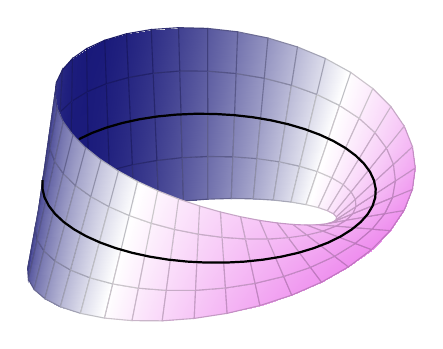
\begin{tikzpicture}
			\begin{axis}[
			  hide axis,
			  view = {40}{40}
			]
			\addplot3 [
			  surf,
			  colormap/violet,
			  shader     = faceted interp,
			  point meta = x,
			  samples    = 40,
			  samples y  = 5,
			  z buffer   = sort,
			  domain     = 0:360,
			  y domain   =-0.5:0.5
			] (
			  {(1+0.5*y*cos(x/2)))*cos(x)},
			  {(1+0.5*y*cos(x/2)))*sin(x)},
			  {0.5*y*sin(x/2)}
			);
		  
			\addplot3 [
			  samples=50,
			  domain=-145:180, % The domain needs to be adjusted manually,
							   % depending on the camera angle, unfortunately
			  samples y=0,
			  thick
			] (
			  {cos(x)},
			  {sin(x)},
			  {0}
			);
			\end{axis}
		  \end{tikzpicture}
		  \caption{Nastro di Möbius. La circonferenza disegnata serve proprio per far vedere che un giro attorno a questo nastro inverte l'orientazione: se io prendessi un versore normale "puntato" verso l'esterno, allora dopo un giro questo sarebbe invertito, dunque ci sarebbe una discontinuità e $\nu$ non sarebbe continua,
		  come richiesto dalla definizione di superficie orientabile}
	\end{figure}
\end{remark}
\begin{example}[esempio di calcolo del flusso attraverso una superficie] \hspace{1cm} \\
	Sia $T=\left\{(x, y, z) \in \mathbb{R}^3: x, y, z > 0, x + \frac{y}{2}+\frac{z}{4}=1 \right\}$ e $F(x, y, z)=(y, x, \frac{z}{2}+ y - 2)$. Calcolare il flusso attraverso questa superficie
\end{example}
\begin{proof}[Svolgimento]
	Osserviamo che, essendo il triangolo un piano "confinato" a $x, y, z > 0$, possiamo facilmente trovare il versore normale prendendo il vettore $(1, \frac{1}{2}, \frac{1}{4})$. Possiamo altrimenti porre
	$g(x, y, z) = x + \frac{y}{2} + \frac{z}{4}$ e definire il nostro triangolo tramite la funzione definente $g$: lo spazio tangente ad ogni punto $x_0$ di questa superficie sarà dato da $\nabla g(x_0) = (1, \frac{1}{2},\frac{1}{4})$. \\
	Esplicitiamo la $x$:
	$$
	x = 1 - \frac{y}{2} - \frac{z}{4} > 0 \text{ siccome } 0 < x = 1 - \frac{y}{2} - \frac{z}{4} = \varphi(y, z)
	$$
	La normale a questo piano è dato naturalmente dal gradiente che corrisponde proprio a
	$$
	\nabla g(x, y, z) = \begin{pmatrix} 
		\partial_y \varphi & \partial_z \varphi \\
		1 & 0 \\
		0 & 1
	\end{pmatrix} \implies |\nabla g| = \sqrt{(\partial_y \varphi)^2 + (\partial_z \varphi)^2 + 1} = \sqrt{1 + |\nabla \varphi|^2} 
	$$
	dunque il vettore normale è proprio
	$$
	\nu = \frac{(1, \frac{1}{2}, \frac{1}{4})}{\sqrt{1 + (\frac{1}{2})^2 + (\frac{1}{4})^2}} \implies \Phi(F, \Sigma, \nu) = \int_H \innerprod{F}{\frac{\nabla g}{\sqrt{1 + |\nabla \varphi|^2}}} \sqrt{1 + |\nabla \varphi|^2} dydz
	$$
	dove $H = \{(y, z) \in \mathbb{R}^2 : 0 < \frac{y}{2} + \frac{z}{4} < 1 \}$. Dunque
	$$
	\int_H \innerprod{F}{(1, \frac{1}{2}, \frac{1}{4})} dydz =	\int_0^2 y \int_0^{4 - 2y} dzdy = \frac{8}{3}
	$$
\end{proof}

\subsection{Frontiera regolare di un aperto}

\begin{definition}[punto regolare di frontiera e derivata esterna] \hspace{1cm} \\
	Sia $\Omega \subseteq \mathbb{R}^3$ un insieme aperto. Diremo che $x \in \text{Fr} \, \Omega$ è un punto di frontiera regolare se
	\begin{enumerate}[label=\protect\circled{\arabic*}]
		\item $\exists O \subseteq \mathbb{R}^3$ aperto tale che $x \in O \cap \text{Fr} \, \Omega$
		\item $\exists g \in C^1(O)$ tale che $O \cap \Omega = \{y \in O : g(y) < 0 \}$
		\item $\nabla g(y) \neq 0 \, \, \forall y \in O$
	\end{enumerate}
	Denoteremo con $\partial_{\text{reg}}$ la frontiera regolare o bordo regolare di $\Omega$. Diremo che $g$ definisce una porzione di frontiera regolare
	$O \cap \text{Fr} \, \Omega$ e
	$$
	\nu(y) = \frac{\nabla g(y)}{|\nabla g(y)|} \, \, \forall y \in O \cap \text{Fr} \, \Omega
	$$
	dove $\nu: \partial_{\text{reg}} \Omega \mapsto \mathbb{S}^2$ è detta normale esterna ad $\Omega$ in $x \in \partial_{\text{reg}} \Omega$.
\end{definition}
\begin{remark}
I punti regolari di frontiera sono quei punti che separano l'interno dall'esterno. Fare riferimento alla seguente immagine
\begin{figure}[H]
    \centering
    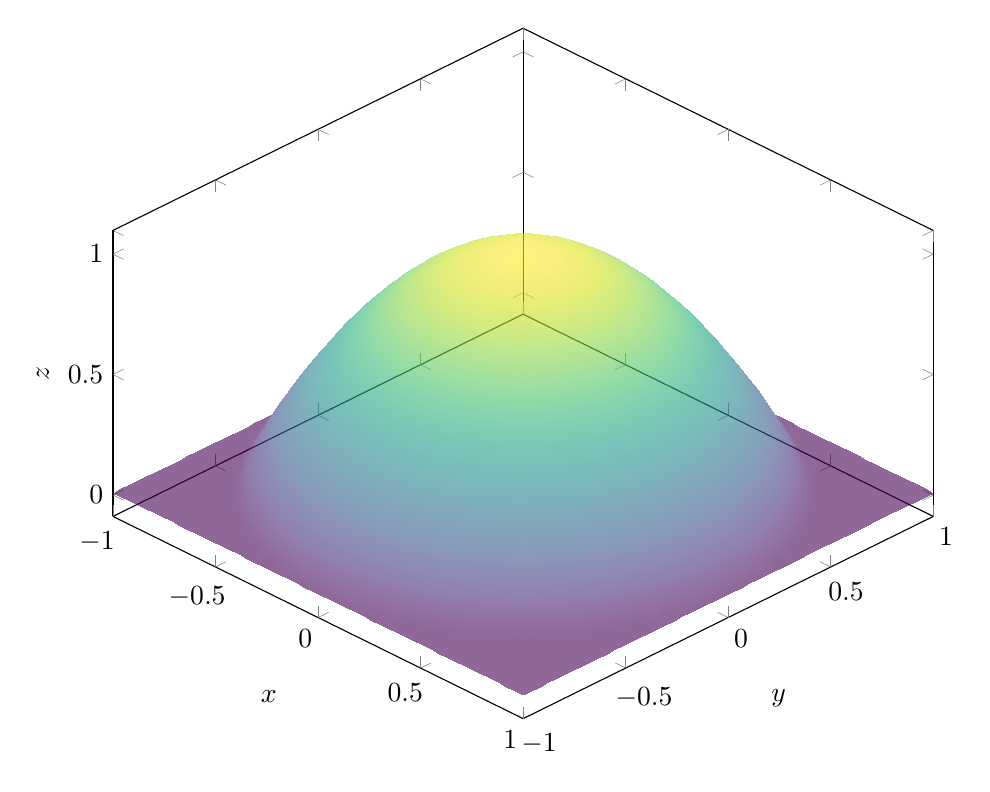
\begin{tikzpicture}
        \begin{axis}[
            width=12cm,
            view={45}{45},        % Angolazione della vista
            xlabel={$x$},         % Etichetta asse x
            ylabel={$y$},         % Etichetta asse y
            zlabel={$z$},         % Etichetta asse z
            domain=-1:1,          % Limiti degli assi x
            y domain=-1:1,        % Limiti degli assi y
            samples=50,
            clip=false,           % Disabilita il clipping
            z buffer=sort
        ]
        % Grafico della superficie limitato alla regione z > 0.01
        \addplot3[
            surf,
            opacity=0.6,          % Riduci l'opacità
            shader=interp,
            colormap/viridis,     % Sfumatura di colori più delicata
        ]
        {max(0.01, 1 - x^2 - y^2)}; % Imposta un valore minimo di z
        \end{axis}
    \end{tikzpicture}
\end{figure}
\end{remark}
\begin{prop}
	Dato $\Omega \subseteq \mathbb{R}^3$ il sottoinsieme $\partial_{\text{reg}} \Omega$ di $\text{Fr} \, \Omega$ è un'unione al più numerabile di superfici regolari.
\end{prop}
\begin{proof}[Idea della dimostrazione]
Si osserva che $\partial_{\text{reg}} \Omega$ è un'aperto in $\text{Fr} \, \Omega$ rispetto la topologia (indotta) di sottospazio e che tale topologia ha una base numerabile di aperti, dunque per il teorema di Lindelöf ogni ricoprimento aperto
ha un sottoricoprimento numerabile. Prendendo come aperti del ricoprimento di $\partial_{\text{reg}} \Omega$ gli $\{O_x : x \in \partial_{\text{reg}} \Omega \}$ dove $O_x \subseteq \mathbb{R}^3$ e $g: O_x \to \mathbb{R}$ definisce $\partial_{\text{reg}} \Omega$
intorno a $x$, dunque la tesi.
\end{proof}
\begin{prop}
Se $\nu: \partial_{\text{reg}} \to \mathbb{S}^2$ è la normale esterna allora è continua
\end{prop}
\begin{proof}
$$
\nu(y) = \frac{\nabla g(y)}{|\nabla g(y)|} \, \, y \in O \cap \text{Fr} \, \Omega
$$
è continua sulla porzione di frontiera $O \cap \text{Fr} \, \Omega$ siccome rapporto di funzioni continue
\end{proof}
Presa una funzione $F: \mathbb{R}^3 \to \mathbb{R}^3$ possiamo allora definire il flusso, supponendo che $\int_{\partial_{\text{reg}}} |F| < +\infty$ (ovvero $F$ è $\sigma-$integrale su $\partial_{\text{reg}}$), attraverso la frontiera regolare
$$
\Phi(F, \partial_{\text{reg}} \Omega, \nu) = \int_{\partial_{\text{reg}} \Omega} \innerprod{F}{\nu} d \sigma
$$
\begin{definition}[divergenza]
	Sia $F \in C^1(\Omega, \mathbb{R}^3), \Omega \subseteq \mathbb{R}^3$ aperto, allora definiamo la divergenza di $F$ la funzione scalare
	$$
	\Div F = \partial_x F_x + \partial_y F_y + \partial_z F_z
	$$
	dove $F=(F_x, F_y, F_z)$
\end{definition}
\begin{theorem}[della divergenza]
	Sia $\Omega \subseteq \mathbb{R}^3$ limitato e connesso per archi tale che
	\begin{enumerate}[label=\protect\circled{\arabic*}]
		\item $\sigma(\text{Fr} \, \Omega \setminus \partial_{\text{reg}}) = 0$
		\item $\sigma(\partial_{\text{reg}}) < +\infty$
	\end{enumerate}
	allora se $F \in C^1(\mathcal{U}, \mathbb{R}^3), \bar{\Omega} \subseteq \mathcal{U}$ dove $\mathcal{U} \subseteq \mathbb{R}^3$ è aperto vale la seguente formula
	$$
	\int_\Omega \Div F dm_3 = \int_{\partial_{\text{reg}} \Omega} \innerprod{F}{\nu} d\sigma = \Phi(F, \partial_{\text{reg}} \Omega, \nu)
	$$
\end{theorem}
\begin{example}[calcolo del flusso tramite il teorema della divergenza]
	Calcolare $\Phi(F, \Sigma, \nu)$ dove $F(x, y, z)=(x, y, z)$ e $\Sigma=\{(x, y, z) \in \mathbb{R}^3 : 4x^2 + 4y^2 + z^2 = 4, x \leq 0 \}$, dove questa è orientata dalla normale $\nu$ che è individuata dalla condizione
	$\nu(-1, 0, 0) = (-1, 0, 0)$.
\end{example}
\begin{proof}[Svolgimento]
	Osserviamo che sul semipiano $D = \Sigma \cap \{x = 0\}$ avremo che la normale $\eta = (1, 0, 0)$ mentre per quanto riguarda il resto della superficie dobbiamo essere un po' più originali.
	$$
	\Phi(F, \partial \Omega, n) = \Phi(F, \Sigma, \nu) + \Phi(F, D, \eta) \stackrel{\text{thm divergenza}}{=} \int_\Omega \Div F dm_3 = 3\int_\Omega dm_3 = 3m_3(\Omega) 
	$$
	dove $\Omega = \{(x, y, z) \in \mathbb{R}^3 | 4x^2 + 4y^2 + z^2 < 4, x < 0 \}$. Possiamo fare questo integrale senza problemi in coordinate sferiche
	$$
	m_3(\Omega) = \int_\Omega dxdydz = 2 \int_{\Omega'} dxdydz' = 2 m_3(B(0, 1) \cap \{ x < 0 \})= \frac{4}{3} \pi 
	$$
	dove, per agevolare il calcolo dell'integrale, abbiamo fatto il cambio di coordinate $(x', y', z') \mapsto (x', y', 2z') = (x, y, z)$ dunque il jacobiano di questa trasformazione era pari a $2$ e poi abbiamo diviso per $2$ per ottenere solo metà contributo della sfera (siccome la condizionee $x<0$ taglia metà della sfera).
	Dunque
	$$
	\Phi(F, \Sigma, \nu) = 3m_3(\Omega) = 4\pi
	$$
\end{proof}
Mostriamo due esempi famosi del teorema della divergenza
\subsection{Legge di Gauss}
Sia $E = k_e \frac{q}{r^2}\hat{r}$ il campo elettrico generato da una carica puntiforme, allora
\begin{align*}
&\Div E = \Div(k_e \frac{q}{r^2} \hat{r}) = \Div(k_e \frac{q}{r^3}r) = k_e q \sum_{i=1}^3 \partial_{x_i} (\frac{x_i}{|x|^3}) = k_e q \sum_{i=1}^3 \frac{|x|^3 - 3 x_i^2 |x|}{|x|^6} = \\
&=k_e q \frac{3|x|^2 - 3 |x|^2}{|x|^5} = 0
\end{align*}
$E$ è ben definito $\Omega \setminus B(x_0, \varepsilon)$ e, dunque, possiamo applicare il teorema della divergenza su $\Omega \setminus B(x_0, \varepsilon)$, da cui deduciamo che
\begin{align*}
&\Phi(E, \partial_{\text{reg}} (\Omega \setminus B(x_0, \varepsilon)), \nu) = \int_{\partial \Omega} \innerprod{E}{\nu} d\sigma + \int_{\partial B(x_0, \varepsilon)} \innerprod{E}{\nu} d\sigma = \Phi(E, \partial \Omega, \nu) - k_e \frac{q}{\varepsilon^2} (4 \pi \varepsilon^2) = \\
&=\int_{\Omega \setminus B(x_0, \varepsilon)} \Div E dm_3 = 0 \implies \Phi(E, \partial \Omega, \nu) = 4 \pi k_e q
\end{align*}
dove abbiamo usato il fatto che $\int\limits_{B(x_0, \varepsilon)} \innerprod{E}{\nu} = E 4 \pi \varepsilon^2$ in virtù delle simmetria radiale del campo elettrico.
\subsection{Equazione di continuità in fluidodinamica}
Sia $\Omega$ una regione di spazio di un fluido che sta "uscendo" da questo e indichiamo con $d\Sigma$ l'elemento infinitesimo di superficie, $d\sigma$ l'elemento infinitesimo di area e $v(x, y, z, t)$ la velocità della particella di un liquido nel punto $(x, y, z)$ al tempo $t$. In un tempo
infinitesimale $dt$, l'elemento infinitesimale di volume di liquido passante attraverso l'elemento di superficie $d\Sigma$ è pari a $|\vec{v} \cdot \nu|d\sigma$, dove $\vec{v}$ è la velocità del liquido mentre $\nu$ è la normale alla
superficie. Supponendo che il nostro liquido abbia una densità $\rho(x, y, z, t) \geq 0$ variabile, la quantità di fluido totale è data da
$$
V = \int_\Sigma \rho (\vec{v} \cdot \nu)d\sigma = \Phi(\rho \vec{v}, \Sigma, \nu) 
$$
Per la conservazione della massa dobbiamo avere che
$$
\frac{M_t - M_{t+dt}}{dt} = V
$$
ma sapendo che $M_t = \int\limits_\Omega \rho(x, y, z, t) dxdydz$ (ovvero la massa di tutto il fluido è l'integrale in tutta la regione di spazio $\Omega$ in cui si trova il fluido al tempo $t$), allora
$$
-\frac{\partial}{\partial t} \int_\Omega \rho(x, y, z, t)dxdydz = \int_{\partial \Omega} \rho \vec{v} \cdot \nu d\sigma
$$
dove il $-$ deriva dal fatto che la $V$ è naturalmente positiva ma il bilancio di massa dove che il fluido esce dalla superficie diminuisce, dunque la derivata è negativa. Tramite la teoria di Lebesgue è possibile portare la derivata all'interno dell'integrale con ipotesi deboli, dunque
$$
\int_\Omega - \frac{\partial \rho}{\partial t} dm_3 = \Phi(\rho \vec{v}, \partial \Omega, \nu) \stackrel{\text{thm divergenza}}{=} \int_\Omega \Div(\rho \vec{v}) \implies \frac{\partial \rho}{\partial t} + \Div(\rho \vec{v}) = 0
$$
che prende il nome di equazione di continuità.

\section{Teorema del rotore}
Vogliamo adesso enunciare il teorema del rotore. Ci limiteremo all'enunciato relativo alle superfici elementari, ma naturalmente è possibile mostrare la sua valenza anche per superfici più "generali". Prima di fare ciò è necessaria e, soprattutto, doverosa qualche definizione.
\subsection{Superfici elementari}
\begin{definition}[curva regolare a tratti]
	Una curva $\gamma: [a, b] \to \mathbb{R}^n$ si dice regolare a tratti se $\gamma \in C^1_\text{tratti}$ e $\dot{\gamma}(t) \neq 0 \, \, \forall t \in (t_{i-1}, t_i) \, \, \forall i \in \{1, \ldots, N \}$ dove $a=t_0 < t_1 < \ldots < t_{N-1} < t_N = b$ è il partizionamento che rende $\gamma$ $C^1_\text{tratti}$. Se $N=1$, ovvero $t_0=a$ e $t_1=b$ diremo che $\gamma$ è regolare.
\end{definition}
\begin{definition}[dominio piano elementare]
	Un insieme $H \subseteq \mathbb{R}^2$ è detto dominio piano elementare se è limitato e la sua frontiera $\partial H$ è una curva semplice, chiusa e regolare a tratti 
\end{definition}
\begin{remark}
Il "bordo" di questo dominio può essere frastagliato in alcuni punti
\begin{figure}[H]
	\centering
	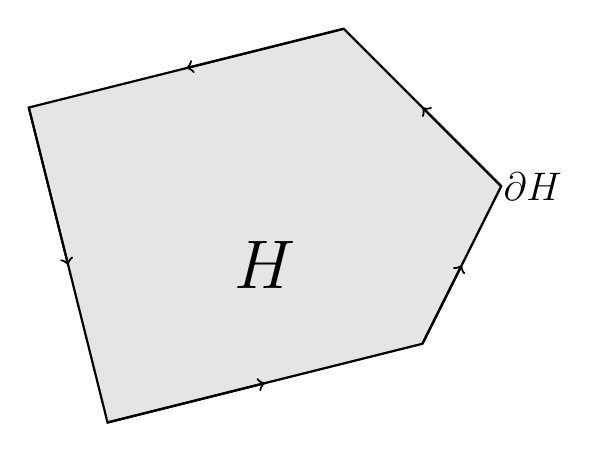
\begin{tikzpicture}[scale=2]
		\filldraw[fill=gray!20, draw=black, thick] 
			(0, 0) -- (2, 0.5) -- (2.5, 1.5) -- (1.5, 2.5) -- (-0.5, 2) -- cycle;
		
		% Etichetta della regione H
		\node at (1, 1) {\Huge $H$};
	
		% Disegna la frontiera con frecce per l'orientamento
		\draw[->, thick] (0, 0) -- (1, 0.25);
		\draw[->, thick] (2, 0.5) -- (2.25, 1);
		\draw[->, thick] (2.5, 1.5) -- (2, 2);
		\draw[->, thick] (1.5, 2.5) -- (0.5, 2.25);
		\draw[->, thick] (-0.5, 2) -- (-0.25, 1);
	
		% Etichetta della frontiera
		\node at (2.7, 1.5) {\Large $\partial H$};
	
		% Disegna una curva rossa tra due punti adiacenti sulla frontiera
		%\draw[thick, red] (2, 0.5) to[out=120, in=240] (2.5, 1.5);
	
		% Punti di partenza e arrivo della curva
		%\filldraw[red] (2, 0.5) circle (0.05);   % Punto iniziale
		%\filldraw[red] (2.5, 1.5) circle (0.05); % Punto finale
	
		% Aggiungi un clip per evitare che il riempimento si estenda oltre la curva rossa
		\clip (0, 0) -- (2, 0.5) -- (2.5, 1.5) -- (1.5, 2.5) -- (-0.5, 2) -- cycle;
	\end{tikzpicture}
	\caption{Esempio di dominio piano elementare. Come si vede il bordo è frastagliato, eppure è possibile parametrizzare il bordo con una curva semplice, chiusa e regolare a tratti}
\end{figure}
\end{remark}
Tramite i domini elementari possiamo definire le superfici elementari
\begin{definition}[superficie elmentare]
	Diremo che $\Sigma \subseteq \mathbb{R}^3$ è una superficie elementare se esiste un dominio piano elementare $H \subseteq \mathbb{R}^2, \mathcal{U} \subseteq \mathbb{R}^2$ aperto e una funzione $\Phi: \bar{H} \to \mathbb{R}^3$ tali che
	\begin{enumerate}[label=\protect\circled{\arabic*}]
		\item $\Phi$ è iniettiva su $\bar{H}$, $\bar{H} \subset \mathcal{U}$, $\Phi \in C^1(\mathcal{U}, \mathbb{R}^3)$;
		\item $d\Phi: \mathbb{R}^2 \to \mathbb{R}^3$ è iniettivo $\forall u \in \bar{H}$;
		\item $\Sigma = \Phi(H)$.
	\end{enumerate}
	Inoltre, diremo che $\Phi$ è una parametrizzazione di $\Sigma$, $\bar{\Sigma} = \Phi(\bar{H})$ è la chiusura di $\Sigma$ pertanto, posto $\partial \Sigma = \Phi(\partial H)$, avremo che
	\begin{equation}
		\bar{\Sigma} = \Sigma \cup \partial \Sigma
	\end{equation}
\end{definition}
\begin{remark}
	La condizione $\Phi(\partial H) = \partial \Sigma$ serve per evitare delle situazioni come il grafico dell'\emph{otto}: possiamo parametrizzare un $8$ solo per $y>0$ ma in $z=0$, se invertiamo la funzione localmente, possiamo estenderla anche al semipiano inferiore ottenendo qualcosa che non è più un $(x, y)-$grafico.
\end{remark}
\begin{remark}
Possiamo mostrare che una superficie elementare è una superficie regolare, siccome $\Sigma$ è localmente un grafico. Infatti
$$
D\Phi(u) = \begin{pmatrix}
\nabla \Phi_1(u) \\
\nabla \Phi_2(u) \\
\nabla \Phi_3(u)
\end{pmatrix}
$$
e supponiamo che $M_{\text{12}}(D\Phi) = \det \begin{bmatrix} \nabla \Phi_1 \\ \nabla \Phi_2 \end{bmatrix} \neq 0$: possiamo considerare $\Phi_{(1, 2)}: U \to \mathbb{R}^2$ tale che $u \mapsto (\Phi_1(u), \Phi_2(u))$. Per ipotesi avremo che $\det D\Phi_{(1, 2)}(u) = M_{12}(D\Phi(u)) \neq 0 \implies$ per il teorema della funzione inversa $\exists \delta > 0: \exists V \subseteq \mathbb{R}^2: \Phi_{(1,2)}: B(u, \delta) \to V$ invertibile con inversa $\Psi: V \to B(u, \delta) \in C^1(V, B(u, \delta))$.
Ma allora $(\Phi \circ \Psi)(u) = (\Phi_1(\Psi(v)), \Phi_2(\Psi(v)), \Phi_3(\Psi(v))) = (\Phi_{(1,2)}(\Psi(v)), \Phi_3(\Psi(v))) = (v, \Phi_3(\Psi(v)))$ siccome $\Psi = \Phi_{(1,2)}^{-1}$. A questo punto possiamo localmente vedere questa superficie elementare come quella che soddisfa l'equazione $z = \Phi_3(\Psi(v))$ e, ponendo $g = \Phi_3 \circ \Psi$, avremo la seguente equazione definente $z=g(v) \implies z - g(v) = 0 \implies \Sigma=f^{-1}(0)$ dove $f(v, z) = z - g(v)$.
\end{remark}
Le superfici elementari "non hanno buchi", ovvero sono degli insiemi semplicemente connessi: consideriamo una curva $\gamma: [a,b] \to \Sigma$ chiusa, allora possiamo considerare la composizione $\Phi^{-1} \circ \gamma : [a, b] \to \bar{H}$ e, siccome $\Phi$ è iniettiva su $\bar{H}$, avremo che la curva $\Phi \circ \gamma$ è anch'essa una curva chiusa. Ma allora sappiamo che $\exists x_0 \in \bar{H} : \exists \mathcal{H} : [0, 1] \times [a, b] \to \bar{H} : \mathcal{H}(0, \cdot) = \Phi^{-1} \circ \gamma(\cdot), \mathcal{H}(1, \cdot) = x_0$, da cui si deduce che
la funzione $\Phi \circ \mathcal{H} : [0, 1] \times [a, b] \to \Sigma$ è una funzione continua tale che $\Phi \circ \mathcal{H}(0, \cdot) = \gamma(\cdot), \Phi \circ \mathcal{H}(1, \cdot) = \Phi(x_0)$ e $\forall t, \mathcal{H}(t, a) = \mathcal{H}(t, b) \implies \Phi \circ \mathcal{H}(t, a) = \Phi \circ \mathcal{H}(t, b)$ per l'iniettività di $\Phi$. La funzione $\Phi \circ H$ è allora è un'omotopia di $\gamma$ in $\Phi(x_0)$.
\begin{prop}
	Se $\gamma \in C^1(\mathcal{U}), \mathcal{U} \subset \mathbb{R}^2$ aperto, $H \subset \mathbb{R}^2$ è un dominio piano elementare e $\bar{H} \subset \mathcal{U}$, allora $\Phi(x, y) = (x, y, \varphi(x, y)), (x, y) \in \mathcal{U}$ definisce una superficie regolare $\Sigma = \Phi(\mathcal{U})$ che è il grafico di $\varphi$ su $\mathcal{U}$.
\end{prop}
\begin{proof}
Osserviamo banalmente che le condizioni $\circled{1}$, $\circled{2}$ della definizione di superficie regolare sono verificate, mentre l'ultima condizione segue da come è stata definita $\Sigma$.
\end{proof}
\begin{remark}
	E' facile osservare che la proposizione $1$ si può formulare analogamente per i casi in cui $\Phi(x, z) = (x, \varphi(x, z), z), (x, z) \in \bar{H}$ e $\Phi(y, z) = (\varphi(y, z), y, z), (y, z) \in \bar{H}$.
\end{remark}
Possiamo a questo punto definire il concetto di normale esterna
\begin{definition}[normale esterna]
	Sia $H \subseteq \mathbb{R}^2$ aperto un dominio piano elementare e sia $\gamma : [a, b] \to \partial H$ una curva semplice, chiusa e regolare a tratti rispetto a $a = t_0 < t_1 < \leq < t_k = b$ la cui immagine è il bordo $\partial H$. Possiamo inoltre assumere che $\gamma$ orienti la curva positivamente, ovvero 
	percorre $H$ lasciandolo a sinistra. Definiamo la normale esterna come
	\begin{align*}
	&\eta(\gamma(t)) = \frac{R\dot{\gamma}(t)}{|R\dot{\gamma}(t)|} & &\forall t \in (t_{j-1}, t_j) \, \forall k \in \{1, \ldots, k \}
	\end{align*}
	dove $R$ è la matrice di rotazione $\frac{\pi}{2}$ in senso orario.
\end{definition}
\begin{figure}[H]
	\centering
	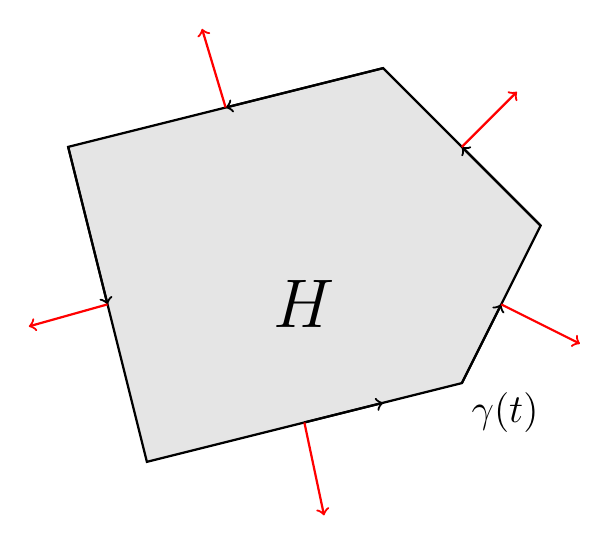
\begin{tikzpicture}[scale=2]
		% Regione H
		\filldraw[fill=gray!20, draw=black, thick] 
			(0, 0) -- (2, 0.5) -- (2.5, 1.5) -- (1.5, 2.5) -- (-0.5, 2) -- cycle;

		% Etichetta della regione H
		\node at (1, 1) {\Huge $H$};

		% Frontiera con frecce per l'orientamento
		\draw[->, thick] (0 + 1, 0+0.25) -- (1+0.50, 0.25+0.125);
		\draw[->, thick] (2, 0.5) -- (2.25, 1); 
		\node[anchor=north west] at (2, 0.5) {\Large $\gamma(t)$};
		\draw[->, thick] (2.5, 1.5) -- (2, 2);
		\draw[->, thick] (1.5, 2.5) -- (0.5, 2.25); % vettore in alto
		\draw[->, thick] (-0.5, 2) -- (-0.25, 1); 

		% Vettori normali esterni ortogonalizzati
		\draw[->, red, thick] (1, 0.25) -- (1.125, -0.34); % Normale esterna in basso (rotazione 90°)
		\draw[->, red, thick] (2.25, 1) -- (2.75, 0.75);  % Normale esterna a destra
		\draw[->, red, thick] (2, 2) -- (2.35, 2.35);    % Normale esterna in alto a destra
		\draw[->, red, thick] (0.5, 2.25) -- (0.35, 2.75); % Normale esterna in alto a sinistra
		\draw[->, red, thick] (-0.25, 1) -- (-0.75, 0.86);  % Normale esterna a sinistra

		% Clip per mantenere il riempimento
		\clip (0, 0) -- (2, 0.5) -- (2.5, 1.5) -- (1.5, 2.5) -- (-0.5, 2) -- cycle;
	\end{tikzpicture}
	\caption{Normale esterna nel caso di un dominio piano elementare}
\end{figure}
Consideriamo adesso $\Phi: U \to \mathbb{R}^3$ di classe $C^1$ una parametrizzazione di una superficie elementare $\Sigma = \Phi(H)$ e $H$ un dominio piano elementare. Abbiamo visto dal capitolo \ref{cap:curve_superfici_regolari} che preso $p \in \Sigma$ con $p = \Phi(w), w \in H$ allora abbiamo che lo spazio tangente a $\Sigma$ in $p \in \Sigma$ è dato da
$$
	T_p(\Sigma) = \text{Span} \{\partial_1 \Phi(w), \partial_2 \Phi(w) \}
$$
mentre una normale a $\Sigma$ in $p$ è data da
$$
	\nu(p) = \frac{\partial_1 \Phi(w) \times \partial_2 \Phi(w)}{|\partial_1 \Phi(w) \times \partial_2 \Phi(w)|}.
$$
Possiamo dunque orientare una superficie elementare scegliendo sempre il campo normale
$$
\nu(p) = \frac{\Phi_{u_1} \Phi(\Phi^{-1}(p)) \times \Phi_{u_2} (\Phi^{-1}(p))}{|\Phi_{u_1} \Phi(\Phi^{-1}(p)) \times \Phi_{u_2} (\Phi^{-1}(p))|}
$$
\newpage 
\newpage 
\newpage